\documentclass{article}

\usepackage[letterpaper,top=1.5cm,bottom=1.5cm,left=1.5cm,right=1.5cm,marginparwidth=1.5cm]{geometry}

\setlength{\parindent}{0pt}

\usepackage{graphicx}
\usepackage{booktabs}
\usepackage{float} 
\usepackage[colorlinks=true, allcolors=blue]{hyperref}
\usepackage[format=hang,font=small]{caption}

\title{Hierarchical Clustering of Differentially Expressed Genes in Pediatric Acute Lymphoblastic Leukemia (ALL) Patient-Derived Xenografts}
\author{Olivia Fernflores}

\begin{document}
\maketitle

\section{Introduction}
Pediatric Acute Lymphoblastic Leukemia (ALL) is the most common form of leukemia in children and about 30\% pediatric cancers are ALL \cite{ALL}. The dataset I'm using was published in 2011 and contains micro array data from both pediatric ALL patients and pediatric ALL samples transplanted into mice \cite{data}. When this paper was published, cure rates for pediatric ALL were around 80\%, with the other 20\% of patients experiencing relapse \cite{data}. The biggest clinical concern lies in patients who relapse and then have a poor prognosis due to factors such as resistance to treatment methods and fast progression of disease. In the early 2000s, about 10\% of pediatric ALL patients would experience the most severe form of relapse, which occurred early and was associated with about a 5\% chance of survival \cite{data}. For patients at high risk of relapse, early identification of risk was shown to improve outcomes \cite{data}. The difficulty was that classifying patients as high or low risk was prone to error. At the time, about \(\frac{2}{3}\) of patients who experienced the most severe form of relapse were identified as low risk \cite{data}. The paper where I got my data seeks to address some of these concerns by looking at new metrics for identifying patients as high or low risk for severe relapse characterized by rapid progression of disease. 
\\

In this paper, the authors use pediatric ALL samples and transplant into NOD/SCID mice. Once the mice develop ALL, the authors collect micro array gene expression data and classify each mouse as "short" or "long" time to leukemia. In their analysis, they describe a bimodal distribution of the "short" and "long" phenotypes, with one group of mice developing leukemia in less than nine weeks and the other group developing leukemia in 12-26 weeks, causing them to choose a cutoff of 10 weeks for classing each sample as "short" or "long". By tracking the patients whose samples were used for transplant into mice, they show that samples that showed a short time to leukemia in the mice were the same samples associated with patients who relapsed within two years after diagnosis. This suggests that the short time to leukemia phenotype observed in the xenograft mice is related to a clinically concerning phenotype, which motivated their study \cite{data}. Using gene expression data from the xenograft mice, they find a set of genes that are differentially expressed in the short time to leukemia samples compared to the long time to leukemia samples. With just these differentially expressed genes, the authors then implement unsupervised clustering and find two clusters, one containing all the short time to leukemia samples and one containing all the long time to leukemia samples. Furthermore, they validate that this expression profile can successfully identify known early relapse patients using a separate set of patients whose samples were not used for transplantation into mice. This is the basis for the rest of their paper, where they build a classifier that can take a patient sample and classify it as high or low risk of early relapse based on how similar or dissimilar the patient data is to the known signatures of the short and long time to leukemia phenotypes \cite{data}. 
\\

For my project, I attempted to re-create their hierarchical clustering pipeline and reproduce Figure 3A from their paper (Figure 1) \cite{data}. Their figure shows the results of hierarchical clustering based on expression level of differentially expressed genes. The dendrogram on the top of the figure shows where each sample clustered, showing two distinct groups that split at the junction of the short time to leukemia samples with the long time to leukemia samples. 

\begin{figure}[H]
    \centering
    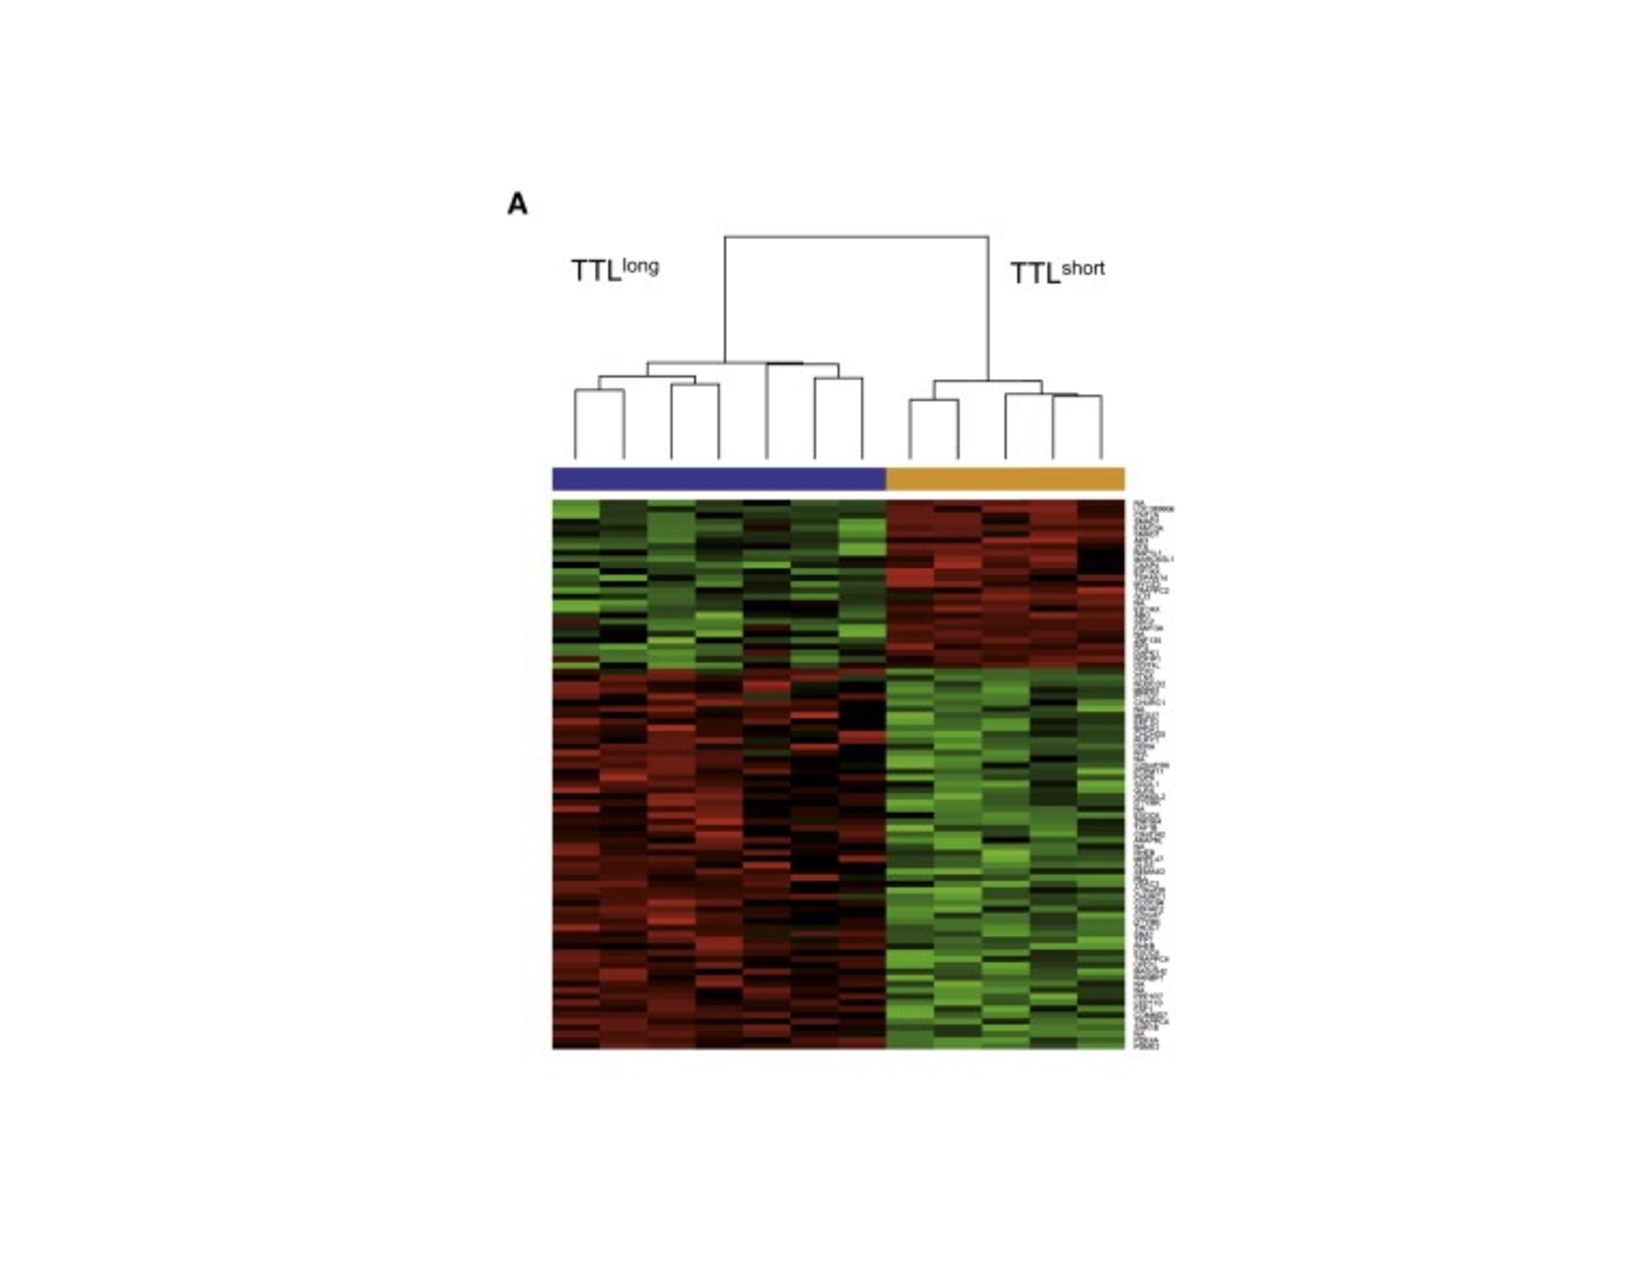
\includegraphics[width=1\textwidth]{/Users/olivia/Documents/Fall 2024/MCB 585/Final Project/report/figure1.pdf}
    \caption{Figure 3A from the original paper. This is the figure I will attempt to produce for my project \cite{data}.}
    \label{fig:1}
\end{figure}

To re-create this figure, I completed the following steps on the xenograft data in R:
\begin{enumerate}
	\item Download, process, and normalize the data
	\item Calculate differential gene expression levels
	\item Filter xenograft data to only include genes with statistically significant differential expression between the short and long time to leukemia samples. 
	\item Perform Principal Component Analysis to check if the data separates into two distinct groups that correspond to the short and long phenotypes
	\item Perform k-means clustering using k = 2 clusters
	\item Perform hierarchical clustering
\end{enumerate}


\section{Results}

\subsection{Differential Gene Expression}
After downloading the dataset from Gene Expression Omnibus, data was separated into xenograft and patient samples, leaving 12 xenograft samples for analysis. Across each of approximately 55000 probes, I calculated differential gene expression between the samples labeled as short time to leukemia and the samples labeled as long time to leukemia (Figure 2). 

\begin{figure}[H]
    \centering
    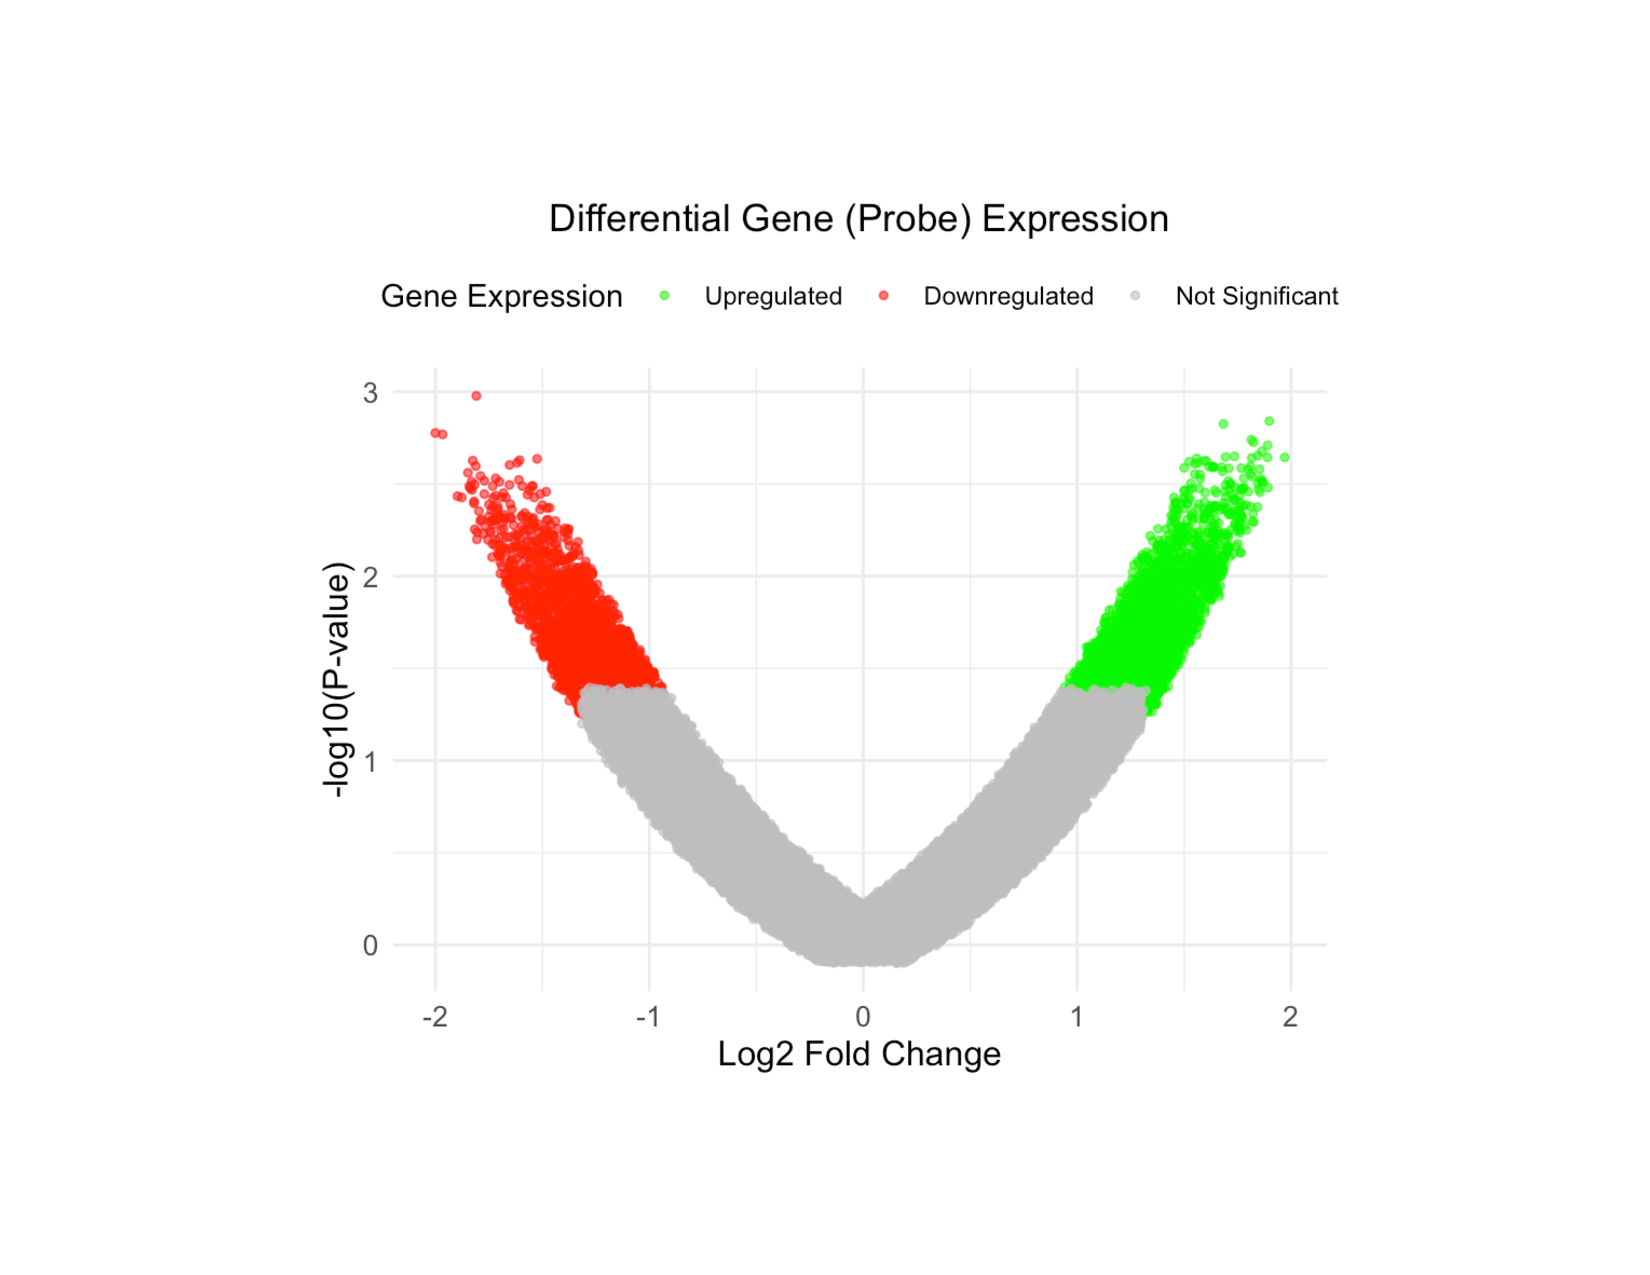
\includegraphics[width=1\textwidth]{/Users/olivia/Documents/Fall 2024/MCB 585/Final Project/report/figure2.pdf}
    \caption{Fold change of gene expression levels between short and long time to leukemia xenograft samples. As in Meyer et. al \cite{data}, 0.05 was used as the p-value for a statistically significant fold change in expression level. Green shows genes that were significantly up regulated in the short time to leukemia xenograft samples, red shows genes that were significantly down regulated in the short time to leukemia xenograft samples. Grey points are not statistically significant at a p value of 0.05}
    \label{fig:2}
\end{figure}

\subsection{Principal Component Analysis}
Before implementing clustering algorithms, I needed to check that the data was actually separable, which I did using principal component analysis (PCA). PCA is a dimensionality reduction technique, which means it can be applied to large datasets (in this case 12 samples x 5575 differentially expressed probes), that reduces datasets to the components contributing most to the overall variance. PCA indicated that along the first principal component, which explains the largest proportion of variance in the overall dataset, samples are easily separable and their separation corresponds to their phenotype of short or long time to leukemia. 

\begin{figure}[H]
    \centering
    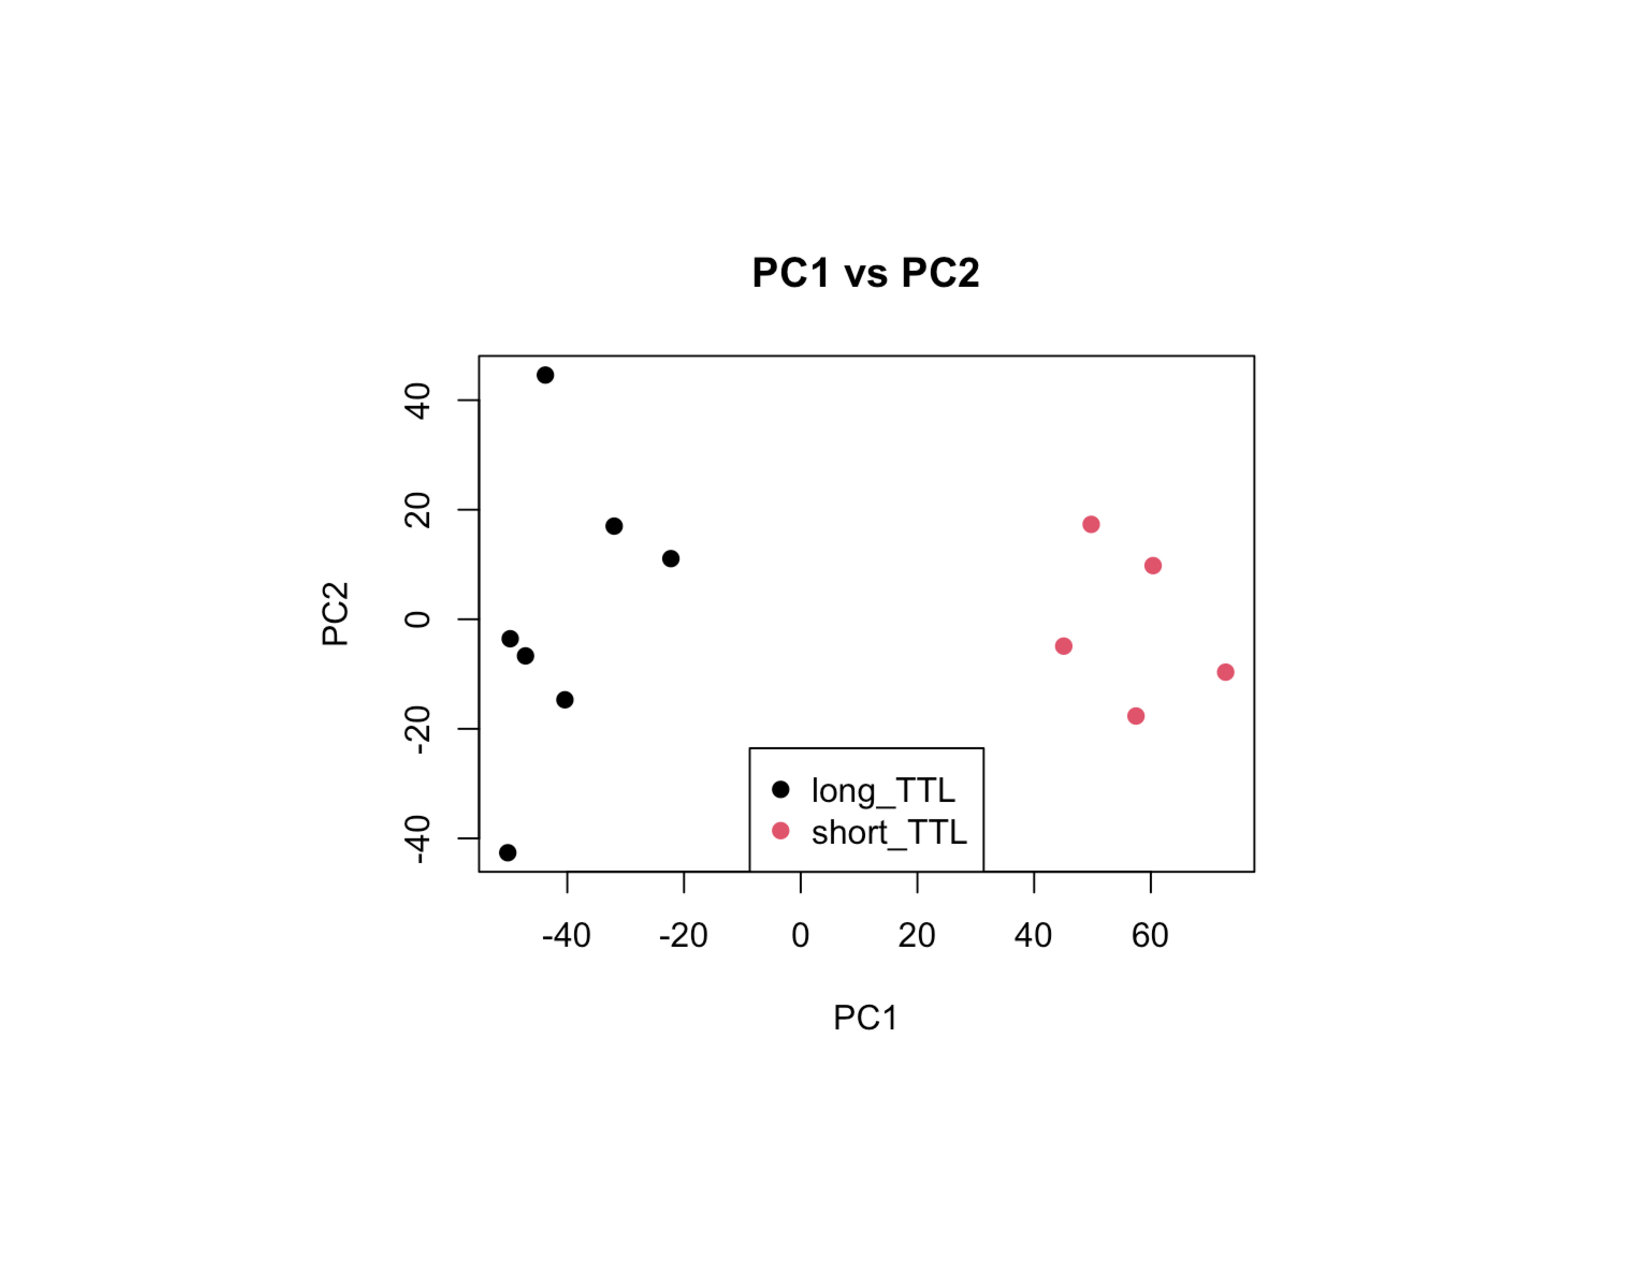
\includegraphics[width=1\textwidth]{/Users/olivia/Documents/Fall 2024/MCB 585/Final Project/report/figure3.pdf}
    \caption{PC1 vs. PC2 using xenograft samples and differentially expressed genes.}
    \label{fig:3}
\end{figure}

\subsection{K-means Clustering}
Confident that my data processing and normalization was reasonable based on the results of PCA, I moved on to implementing K-means clustering. Meyer et. al perform a robust clustering with an underlying K-means framework to show that there are in fact two clusters in the dataset \cite{data}, so I performed a standard K-means clustering using k = 2 clusters (Figure 4) \cite{clust_methods}, \cite{kmeans}. 

\begin{figure}[H]
    \centering
    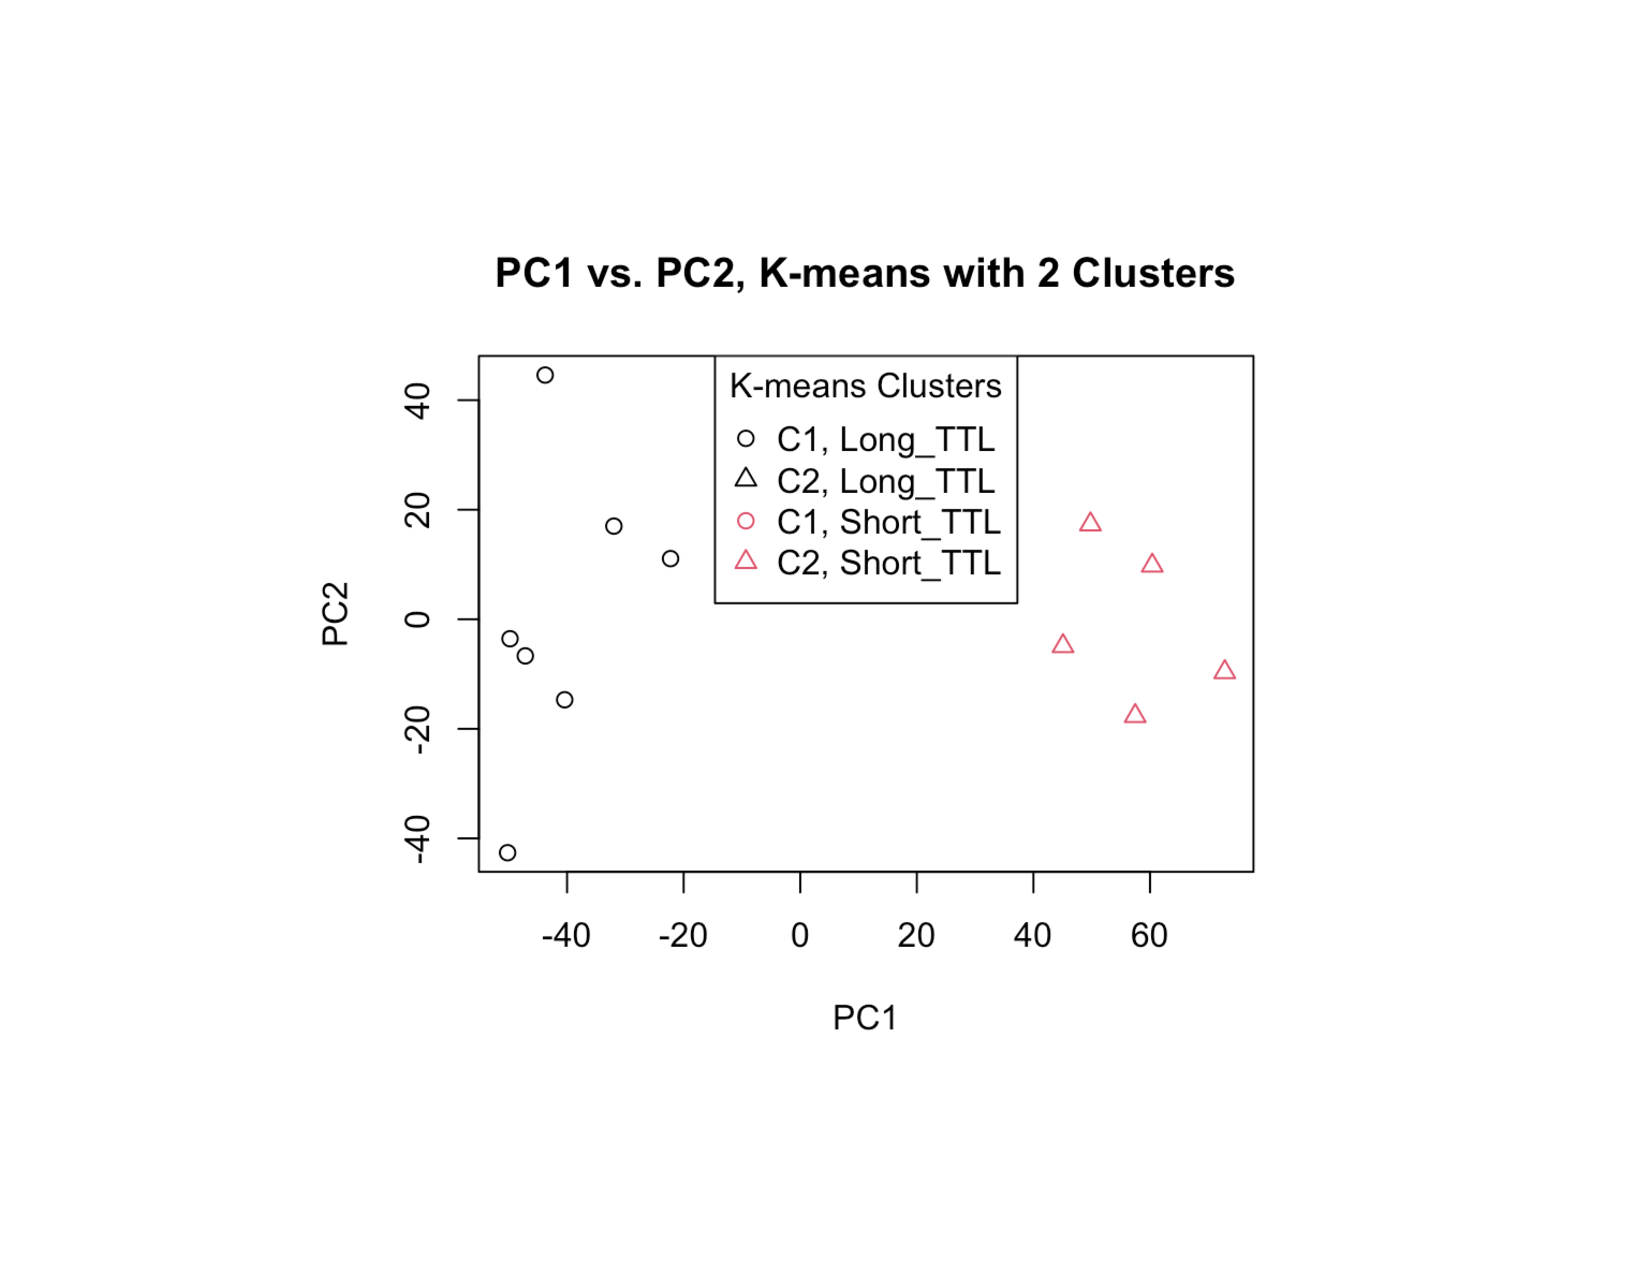
\includegraphics[width=1\textwidth]{/Users/olivia/Documents/Fall 2024/MCB 585/Final Project/report/figure4.pdf}
    \caption{PC1 vs. PC2. Samples are colored according to their phenotype (short or long time to leukemia). Sample shapes represent the cluster assignment after K-means clustering with k = 2 clusters.}
    \label{fig:4}
\end{figure}

As we saw along the first principle component, the data again separates perfectly based on phenotype. All the samples plotted in Figure 4 are either black circles or pink triangles, with the shape representing cluster and the color representing phenotype of short or long time to leukemia. The absence of black triangles and pink circles suggests that the K-means algorithm is assigning samples such that they cluster with other samples of the same experimental phenotype (Figure 4). Although these results were not presented in the original paper, their inclusion here is important validation that the way I processed and normalized the data was reasonable, and suggests that simple clustering methods will perform well to identify relevant differences that contribute to a phenotypic difference, making it reasonable to attempt hierarchical clustering. 

\subsection{Hierarchical Clustering}
Using the same set of genes as the PCA and K-means clustering, I took my xenograft samples and the matrix of their differentially expressed genes and performed hierarchical clustering \cite{clustering}. The resulting dendrogram and gene expression heat map is shown in Figure 5A \cite{hclust}, with the figure from the original paper shown in Figure 5B \cite{data}. 

\begin{figure}[H]
    \centering
    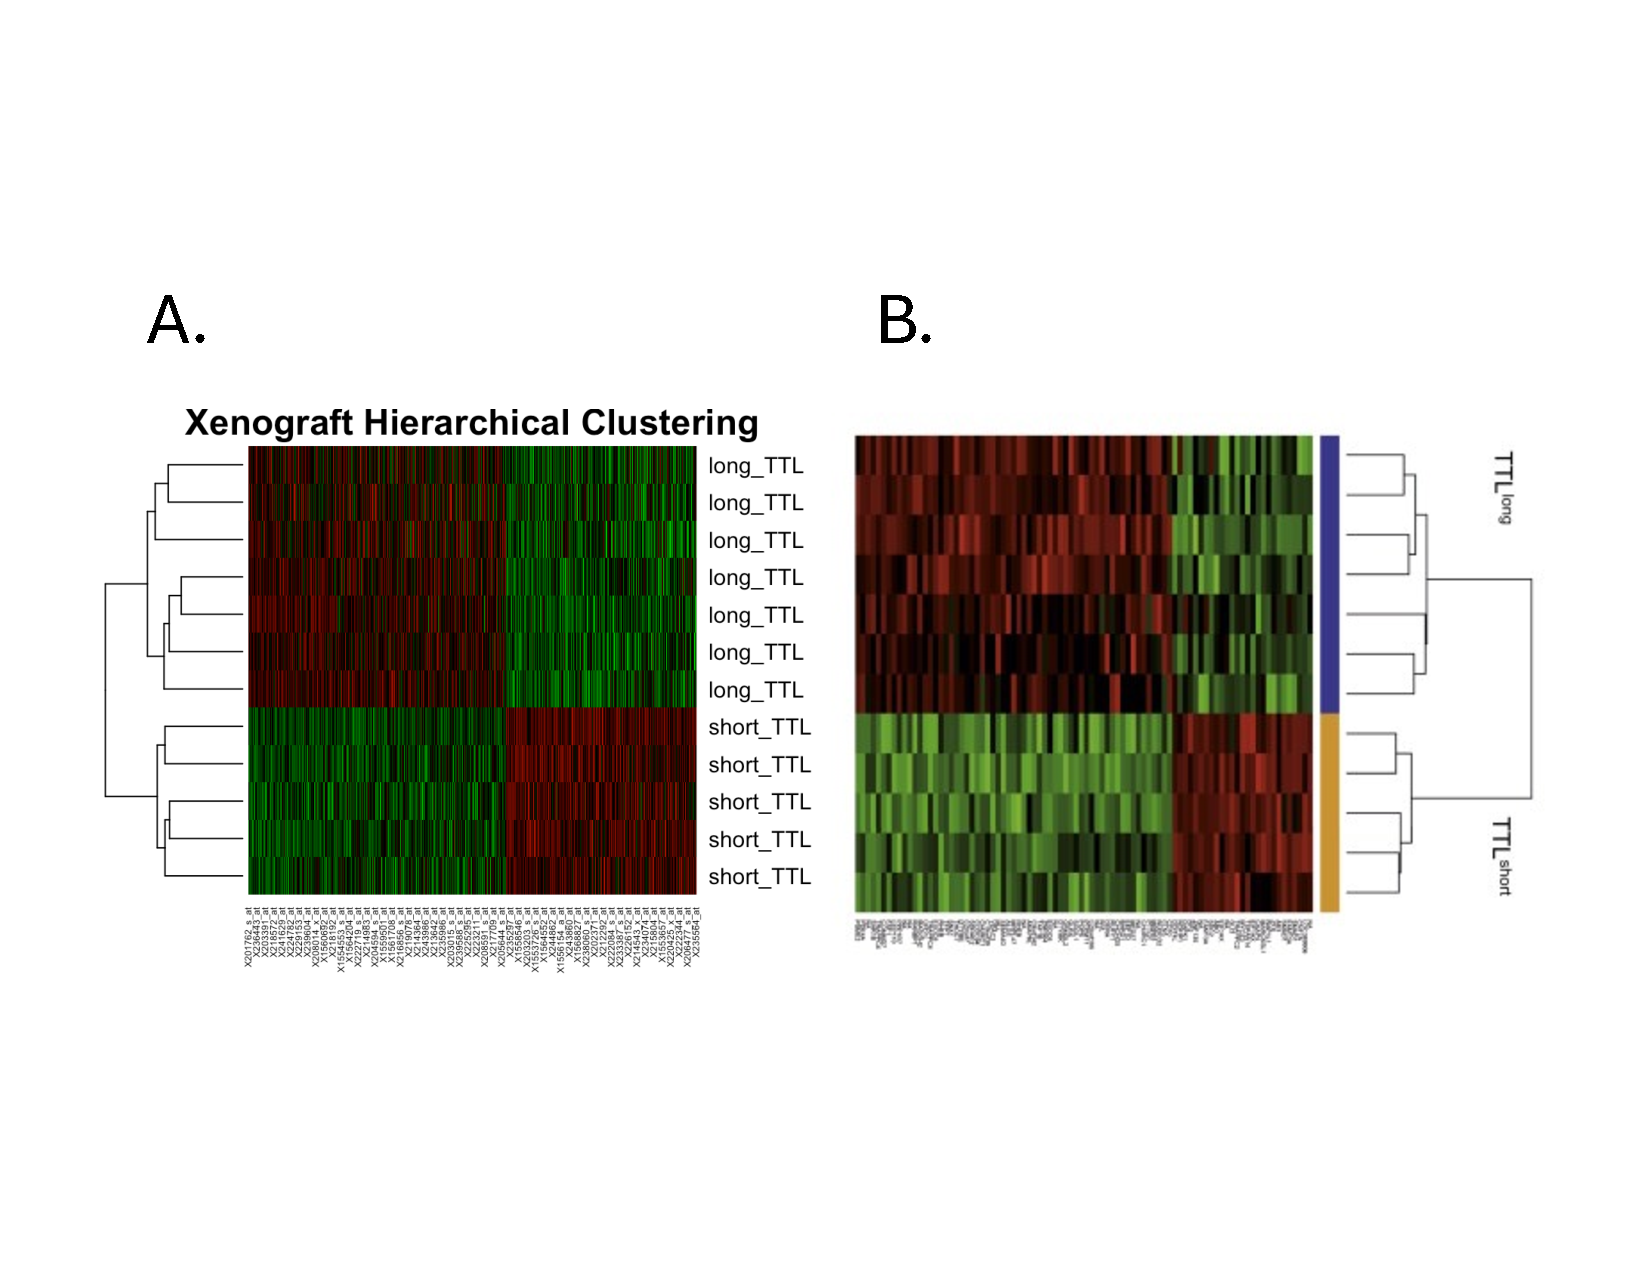
\includegraphics[width=1\textwidth]{/Users/olivia/Documents/Fall 2024/MCB 585/Final Project/report/figure5.pdf}
    \caption{A. Re-produced hierarchical clustering according to methods in the Meyers et al. \cite{data} Dendrogram on left represents the results of hierarchical clustering, true phenotype of samples is labeled on the right. Heat map shows differential gene expression with green and red corresponding to up regulated genes and down regulated genes, respectively, in the short time to leukemia xenografts compared to the long time to leukemia xenografts.
    B. Hierarchical clustering from Meyers et. al \cite{data}. Follows the same color scheme and layout as in A.}
    \label{fig:5}
\end{figure}


\section{Conclusion}
In this project, I successfully re-produced the hierarchical clustering analysis presented in Meyers et. al \cite{data}. Of note is that although I followed the same general steps to Meyers et. al, I had to modify some steps based on what was available in terms of software and current files. For example, Meyers et. al performed a special type of normalization designed explicitly for micro array data \cite{special_normalize}, whereas I used a built-in R function, \textit{scale()} \cite{scale}. I also calculated differential gene expression differently, as the authors were able to implement a method to calculate differential expression across multiple probes for a single gene, whereas I simply calculated differential expression at the level of each individual probe. Despite these methodological differences, the results from hierarchical clustering are almost identical, with the only difference being in the relationship of the four most closely related samples in the long time to leukemia group. Biologically, this difference is not very important, as the primary goal of this clustering is to be able to differentiate between the short and long time to leukemia phenotypes, as the patients from whom those samples were derived had fast and no relapse respectively. The classifier built in Meyers et. al has the goal of improving outcomes by increasing detection accuracy of patients at high risk of relapse, and current statistics about ALL suggest that these efforts moving towards precision medicine have been effective. Recent studies have shown up to 98\% of patients achieving remission \cite{pdq}, and some research hospitals have surival rates as high as 94\% \cite{st.judes}. Compared to a value around 80\% from the early 2010s, these statistics are much better, but there is still more to be done. 
\\




\begin{thebibliography}{10}

\bibitem{ALL} 
Rheingold, Susan R. Acute lymphoblastic leukemia (ALL). Children’s Hospital of Philadelphia. https://www.chop.edu/conditions-diseases/acute-lymphoblastic-leukemia-all.

\bibitem{data}
Meyer, L. H., Eckhoff, S. M., Queudeville, M., Kraus, J. M., Giordan, M., Stursberg, J., Zangrando, A., Vendramini, E., Möricke, A., Zimmermann, M., Schrauder, A., Lahr, G., Holzmann, K., Schrappe, M., Basso, G., Stahnke, K., Kestler, H. A., Kronnie, G. T., & Debatin, K. (2011). Early relapse in ALL is identified by time to leukemia in NOD/SCID mice and is characterized by a gene signature involving survival pathways. Cancer Cell, 19(2), 206–217. https://doi.org/10.1016/j.ccr.2010.11.014

\bibitem{kmeans}
12.5 - R Scripts (K-means clustering) | STAT 897D. (2018). Pennsylvania State University. https://online.stat.psu.edu/stat857/node/125/

\bibitem{clustering}
‌Jin Hwan Do, & Choi, D.-K. (2008). Clustering Approaches to Identifying Gene Expression Patterns from DNA Microarray Data. Molecules and Cells, 25(2), 279–288. https://doi.org/10.1016/s1016-8478(23)17582-0

\bibitem{clust_methods}
‌Altman, N., & Krzywinski, M. (2017). Clustering. Nature Methods, 14(6), 545–546. https://doi.org/10.1038/nmeth.4299

\bibitem{hclust}
‌Hierarchical Clustering in R: Dendrograms with hclust. https://www.datacamp.com/tutorial/hierarchical-clustering-R

\bibitem{special_normalize}
Gautier, L., Cope, L., Bolstad, B.M., and Irizarry, R.A. (2004). affy—analysis of Affymetrix GeneChip data at the probe level. Bioinformatics 20, 307–315.

\bibitem{scale}
scale function - RDocumentation. https://www.rdocumentation.org/packages/base/versions/3.6.2/topics/scale

\bibitem{special_differential}
Opgen-Rhein, R., and Strimmer, K. (2007). Accurate ranking of differentially expressed genes by a distribution-free shrinkage approach. Stat. Appl. Genet. Mol. Biol. 6, Article9.

\bibitem{pdq}
Childhood Acute Lymphoblastic Leukemia Treatment (PDQ®). (2024, October 7). Cancer.gov. https://www.cancer.gov/types/leukemia/hp/child-all-treatment-pdq

\bibitem{st.judes}
Acute lymphoblastic leukemia (ALL) treatment. St. Jude Care & Treatment. https://www.stjude.org/care-treatment/treatment/childhood-cancer/leukemia-lymphoma/acute-lymphoblastic-leukemia-all.html

\end{thebibliography}


\end{document}